\documentclass[]{article}

\usepackage{amsmath}
\setlength{\parindent}{0em}
\setlength{\parskip}{1em}
\usepackage[none]{hyphenat}
\usepackage{fancyhdr}
\usepackage{amssymb}
\usepackage{graphics}
\usepackage{graphicx}
\newcommand{\Lagr}{\mathcal{L}}
\lhead{PHYS - QFT}
\pagestyle{fancy}

\usepackage[top=1.5cm, bottom=1.5cm, left=3cm, right=3cm]{geometry}
\begin{document}
\large

\section*{Overall Notes}

Couple of points in this course where just have to say this is how life is.

Course Structure
\begin{itemize}
	\item Classical Field Theory
	\item QFT, Canonical (second) quantisation.
	\item Interacting Fields, S matrix, perturbation thoery, Feynmann rules.
	\item Quantisation of Dirac, EM fields
	\item QED Feynamm rules, (trace) techniques
	\item Lowest order processes in QED, eg $ee$ scattering.
	\item One loop and higher order processes, renormalisation in scalar fields, lamb shift, g-2.
\end{itemize}

Books:
\begin{itemize}
	\item Peskin \& Schr\"{o}der
	\item Mandl \& Shaw
\end{itemize}

\section{30/9/16 - Preliminaries}	

	\subsection{Why QFT}
	The Schr\"{o}dinger equation is non-relativistic.
	Any attempt to combine QM and Relativity will cause QFT to emerge. 
	The use of QFT and gauge symmetry gives all of physics except gravity.
	
	In field theory we give up the idea of a single particle, we have a field which contains any number of particles. 
	
	SM: $SU(3)xSU(1)xU(1)$
	SU(3): QCD, SU(2): EW, U(1): unification.
	
	All calculations in the SM are done in the framework of QFT.
	
	\subsection{The Emergence of QFT}
	Starting from mass energy equivalence ($E=mc^2$), a massless photon can create an particle antiparticle pair. Vacuum is not "empty", one can pull out particle antiparticle pairs, or an electron can polarise the vaccum to create an ephemeral ee pair.  
	
	This suggests the idea of a field replacement for a single particle.
	
	If one considers an electron in some region of space length $L$, based on the uncertainty principle.
	
	\begin{equation}
		\Delta p.L \sim \hbar \:\:
		\Delta p.c \sim \frac{\hbar c}{L}
	\end{equation}
	If this energy uncertainty exceeds $2m_0c^2$, additional particles can exist within the box. This gives a critical length, $\sim \frac{\hbar}{m_0c}$ which is the Compton wavelength. This compares to the De-Broglie wavelength, and is always smaller than the DB wavelength.
	
	All particles of the same kind are indistinguishable, suggesting the idea of an all pervasive underlying field.
	
	Bose and Fermi statistics will follow from the construction of the field theory.
	
	\subsection{Preliminaries}
	\begin{itemize}
		\item Discard Newtons laws, aside from the action principle and the Euler-Lagrange equations. (massless particles, fields, QM)
	\end{itemize}
	
	\begin{equation}
	S = \int_{t_0}^{t_1}dt\, \Lagr(x, \dot{x}
	\end{equation}
	
	Consider some particle trajectory $X(t)$ and an infinitesimally different trajectory $X'(t)$.
	
	\begin{figure}[h]
	\centering
	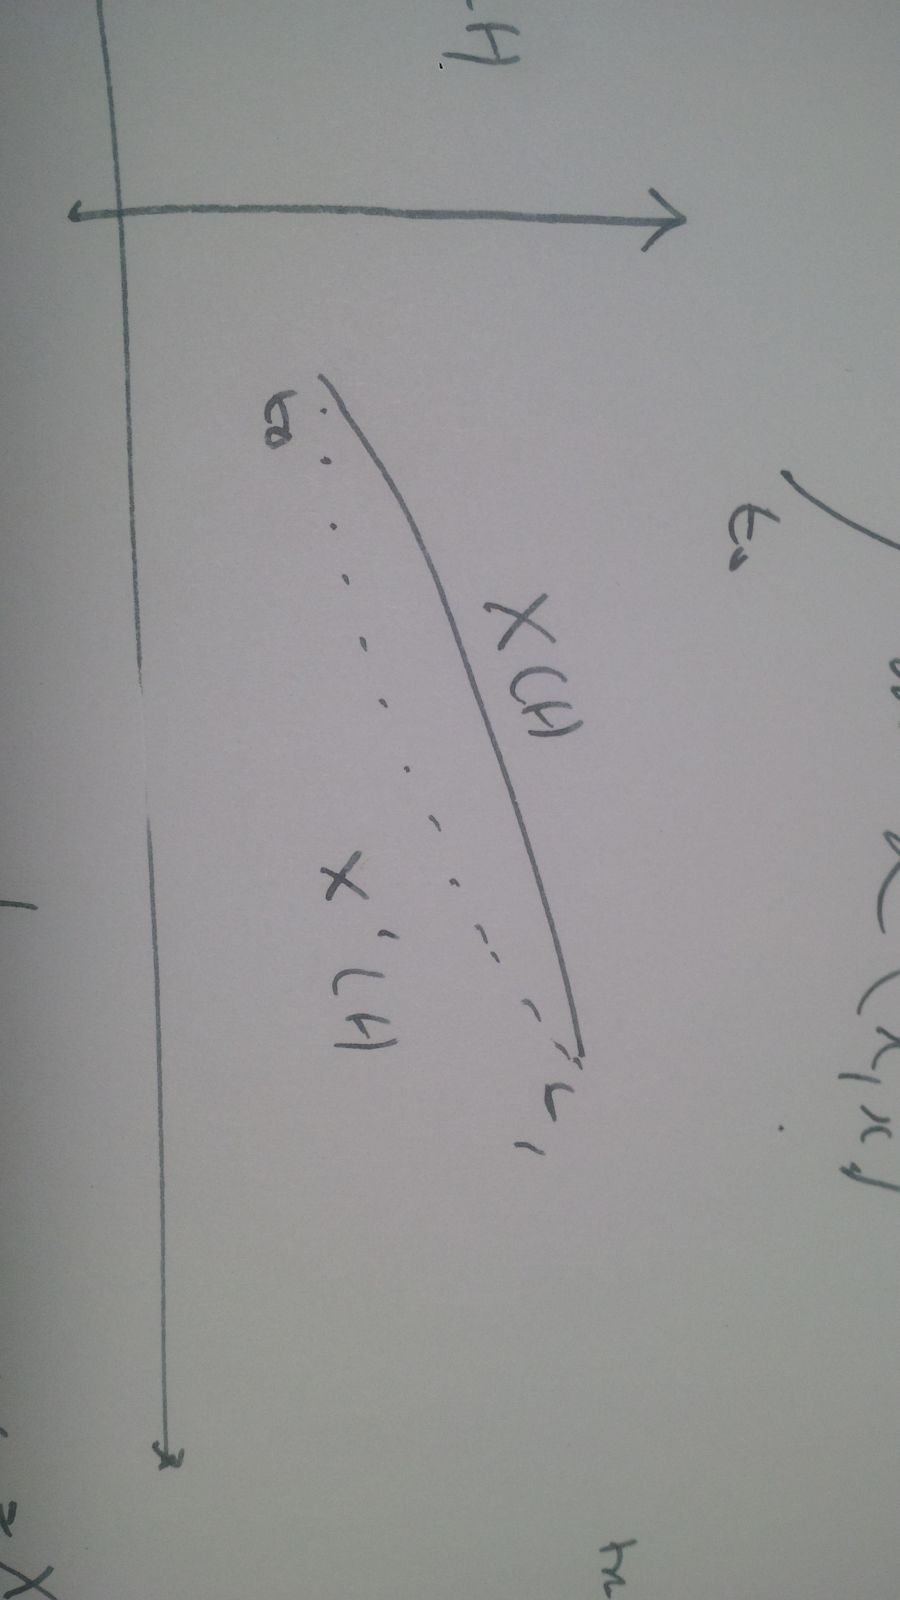
\includegraphics[angle=90,origin=c,width=0.7\linewidth]{trajectory}
	\label{fig:trajectory}
	\end{figure}

	\begin{equation}
	X(t) \rightarrow X(t) + \delta X = X'(t)
	\end{equation}
	
	In this situation $S \rightarrow S + \delta S = \int_{t_0}^{t_1}\Lagr(x + \delta x, \dot{x} + \delta\dot{x})dt$.
	
	\begin{equation}
	S' =  \int_{t_0}^{t_1}\Lagr(x, \dot{x})) + \delta x, \dot{x} + \delta\dot{x})dt
	\end{equation}
	
	For a system with several degrees of freedom $q_i$:
	\begin{equation}
		\frac{partial\Lagr}{\partial q_i}
	\end{equation}
	
	This is equivalent to the Hamiltonian Formalism and the conjugate momentum
	\begin{equation}
	p_i = \frac{\partial\Lagr}{\partial\dot{q_i}}
	\end{equation}
	
	
	Hamiltonian:
	\begin{equation}
	H(q_i, p_i) = p_i\dot{q_i} - \Lagr
	\end{equation}
	
	\subsection{Quantum Mechanics; Second quanitisation}
	
	Take the dynamic variables and replace them with operators:; $x_i \rightarrow \bf{\hat{x_i}}, \bf{p}$


	\section{Lecture 9/10}
	
	\subsection{Interacting fields}
	
	\begin{equation}
		\phi_{in}(x) = \lim\limits_{t\rightarrow-\infty}\phi(x)
	\end{equation}
	\begin{equation}
	\phi_{out}(x) = \lim\limits_{t\rightarrow\infty}\phi(x)
	\end{equation}
	
	Particle tates from vauum
	\begin{equation}
		|p_1,p_2^{in}\rangle = a^\dagger_{in}(p_1)a^\dagger_{in}(p_2)|0\rangle
	\end{equation}
	\begin{equation}
	|k_1,k_2^{out}\rangle = a^\dagger_{out}(k_1)a^\dagger_{out}(k_2)|0\rangle
	\end{equation}
	
	\begin{equation}
	{\langle in|\phi_{in}|in\rangle = \langle out|\phi_{out}|out\rangle}
	\end{equation}
	
	\begin{align}
	|in\rangle = S|out\rangle\\
	|out\rangle = S^-1|in\rangle\\
	S^\dagger S = I\\
	S^\dagger = S^-1\\
	\end{align}
	
	S atric transforms the incoming states to the out going states, where the transofrmation occurs owng to black box proepertie osf the scattering of waves.
	
	\begin{align}
		\phi_{in} = S\phi_{out}S^\dagger \\
		a_{in} = Sa_{out}S^\dagger	
	\end{align}
	
	No interactions implies $S = 1$, so there is no distinction beween in and out basises. WE are intereseted in:
	
	\begin{align}
		\langle f_{out}|i, in\rangle = \langle f_{out}|S|i, out\rangle \\
		\langle f_{in}|S|in\rangle = S_{fi}
	\end{align}
	
	$S_{fi}$ is the scattering amplitude, contains all info on scattering. The scattering matrix $S$ is directly link to $H_{int}$, the interaction Hamiltonian.
	
	\subsection{Dirac tme evolution picture}
	
	Compared to heisenberg or schrodinger. Also called the interaction picture.
	
	$\Phi(\overrightarrow{x}, t) \pi(\overrightarrow{x}, t)$ are Heisenberg pitcutre.
	Operators (time depended):
	\begin{equation}
	\hat{\phi_H}(\vec{x}, t) = e^{iHt}\hat{\phi}_Se^{-iHt} = e^{iHt}e^{-iH_0t}e^{iH_0t}\hat{\phi}_Se^{-iH_0t}e^{iH_0t}e^{-Ht}
	\end{equation}
	
	\begin{equation}
	e^{iH_0t}\phi_Se^{-iH_0t} = \phi_I(\vec{x}, t)
	\end{equation}
	
	which s the interaction or dirac picture.
	
	\begin{align}
	\Phi_H(\vec{x}, t) = U^{-1}(t)\phi_I(\vec{x}, t)U(t) \\
	U(t) = e^{iH_0t}e^{-iHt} \\
	U^\dagger U = I
	\end{align}
	
	U is unitary. We make the following hamiltonian at t = $-\infty$
	
	\begin{align}
	\Phi_{in}(\vec{x}, t) = \Phi_I(\vec{x}, t) = \lim\limits_{t\rightarrow-\infty}\Phi_H\vec{x}, t) \\
	\Phi_{out}(\vec{x}, t) = \Phi_H\vec{x}, t) \:\:as t\rightarrow\infty
	\end{align}
	
	$\Phi_{in} $ and $\Phi_{I}$ are then the same for all times t. $\Phi_I$ always acts on the in basis.
	
	but:
	
	\begin{equation}
	{\Phi_I(\vec{x}, t) = U(t)\Phi_H(\vec{x}, t)U^{-1}(t)}
	\end{equation}
	
	As $t\rightarrow\infty$:
	
	\begin{align}
		\Phi_{in}(\vec{x}, t) = U(t)\Phi_{out}(\vec{x}, t)U^{-1}(t) \\
			\Phi_{in} = U(\infty)\Phi_{out}U^{-1}(\infty) \\
			= U(\infty)\Phi_{out}U^\dagger(\infty) \\
	\end{align}
	
	So, $S = U(\infty) = \lim\limits_{t\rightarrow\infty}U(t)$. considering boundary conditions $U(-\infty) = 1$.
	
	\begin{align}
		i\frac{d}{dt}U(t) = i(e^{iH_0t}(iH_0)e^{-iHt} + e^{iH_0t}e^{-iHt}(-iH) = \\ i^2e^{iH_0t}(H_0 - H)e^{iHt} \\
		=e^{iH_0t}H_{int}e^{-iHt} \\
		= e^{iH_0t}H_{int}e^{-iH_0t}e^{iH_0t}e^{-iHt} \\
		= H_{int}(t)U(t) \\
	\end{align}
	
	$H_{int}$ is an interaction picture operator and depends on $\Phi_{in}$ and $\Pi_{in}$. Solving the equation for U(t):
	\begin{align}
		\int_{-infty}^{t}\frac{d}{dt_1}U(t_1)dt_1 \\ =-i\int_{-\infty}^{t}H_{int}(t_1)U(t_1)dt_1 \\
		U(t) - U(-\infty) = -i\int_{-\infty}^{t}H_{int}(t_1)U(t_1)dt_1 \\
		U(t) = 1 -i\int_{-\infty}^{t}H_{int}(t_1)U(t_1)dt_1  \\
	\end{align}
	
	Try to obtain a series solution t this.
	
	    %\begin{equation}
	    %{\frac{(-i)^n}{n!}\prod_{i=1}^{n}\int_{-\infty}^{t}dt T(H_{int}(t_1) ... H_{int}(t_n))}
	    %\end{equation}
	    
	
	$n^{th}$ term in the series 
	
	    %\begin{align}
	    %(-i)^n\int_{-\infty}^{t}dt_1\int_{-\infty}^{t_1}dt_2 ... \\ int_{-\infty}^{t_{n-1}}H_{int}(t_1) ... \\ H_{int}(t_2)H_{int}(t_n)
	    %\end{align}
	
	Introduce time ordered product of operators:
	
	\begin{align}
	T(\phi(t_1)\phi(t_2)) = \phi(t_1)\phi(t_2) t_1 > t_2 \\
	 \phi(t_2)\phi(t_1) t_2 > t_1 \\
	 \theta(t_1 - t_2)\phi(t_1)\phi(t_2) + \theta(t_2-t_1)\phi(t_2)\phi(t_1) \\
	 \theta(t_a - t_b = 1 (t_a > t_b) or 0(t_b > t_a)
	\end{align}
	
	The $n^{th}$ term can be expressed using T as the time ordering
	

	
	\subsection{S Matrix and Green's function}
	S matrix relates in and out fields, can be written as $S = 1 + iT$. The term 1 corresponds to no scattering. S Matrix will be related to $\langle||T(\phi(x_1)...\phi(x_n))|0\rangle$ I.e. the n point green's function.
	
	Write $|in\rangle$ and $|out\rangle$ states in terms of $a^\dagger_{in}$ etc and hence in terms of fields.
	
	\begin{align}
		S_{fi} = \langle k_1...k_n, out | p_1, p_2, in \rangle \\
		= \langle k_1...k_n, out | a^\dagger_{in}(p_1)|p_2, in\rangle \\
		a^\dagger(q) = i\int d^3\vec{x}(\partial_0e^{-iqx}\phi(x) - e^{-iqx}\partial_0)\\
		a(q) = i\int d^3\vec{x}((\partial_0e^{iqx})\phi(x)  e^{iqx}\partial_0\phi(x))\\
		a^\dagger = -i\int d^3\vec{x}(e^{-qx}\overleftrightarrow{\partial_0}\Phi(x)) \\
		\overleftrightarrow{\partial_0} = \vec{\partial_0} - \overleftarrow{\partial_0} \\
		a(q) = i\int d^3\vec{x}(e^{iqx}\overleftrightarrow{\partial_0}\phi(x)) \\
		S_{fi} = -i\int d^2\vec{x}e^{-ip_1.x_1}\overleftrightarrow{\partial_0}\langle k_1 .. k_n|\phi_in(x)|p_2, in\rangle \\
		=\lim\limits_{min} i\int d^3\vec{x} \\
	\end{align}
	
	\begin{equation}
	S_{fi} =-i\lim\limits_{t_1\rightarrow\infty}\int d^3\vec{x}e^{-ip_1.x_1}\overleftrightarrow{\partial_0}\langle k_1 ... k_n|\phi(x_1)|p_2, in \rangle + i\int_{-\infty}^{\infty}dt_1\frac{\partial}{\partial t_1}(\int d3\vec{x}e^{-ip_1.x_1}\overleftrightarrow{\partial_0}\langle k_1 ... k_n|\phi(x_1)|p_2, in \rangle)
	\end{equation}
	
	Considering the first term:
	
	\begin{align}
	\lim\limits_{t\rightarrow\infty}\int\langle k_1 .. k_n|\phi(x_1)|p_2, in\rangle d^3\vec{x} ... \\
	=  \int\langle k_1 .. k_n, out|\phi(x_{out})|p_2, in\rangle \\
	\propto \int\langle k_1 .. k_n|a^\dagger_{out}}(x_1)|p_2, in\rangle \\
    =\langle 0| a(k_1) ... a(k_n)a^\dagger_{out}(p_1)|p_2, in\rangle
	\end{align}
	
	This equals 0 unless one of the $k_1 ..k_n$ are identical tot the particle $p_1$ does not scatter
	
	\begin{equation}
	S_{fi} = +i\int_{-\infty}^{\infty}dt_1\frac{\partial}{\partial t_1}(\int d^3\vec{x_1}e^{-ip_1.x_1}\overleftrightarrow{\partial_0}\langle k_1 .. k_n|\phi(x_1)|p_2, in\rangle)
	\end{equation}
	
	\begin{equation}
	{ = i\int d^\vec{x}\langle k_1 .. k_n, out|\partial_0(\partial_0(e^{-ip_1.x_1}\phi(x_1) - e^{-ip_1.x_1}\partial_0\phi(x_1))|p_2, in\rangle
	\end{equation}
	
	But
	
	\begin{equation}
		\partial_0((\partial_0e^{-ip_1.x_1}\phi(x_1) - e^{-ip_1.x_1}\partial_0\phi(x_1))
	\end{equation}
	
	\begin{align}
	= E^2(p_1)e^{-ip_1.x_1}\phi(x_1) - e^{-ip_1.x_1}\partial_0^2\phi(x__1)	\\
	= -(((-\vec{\nabla}^2 + m^2)e^{-ip_1.x_1}\phi(x_1) + e^{-ip_1.x_1}\partial_0^2\phi(x_1))
	\end{align}
	
	But 
	
	 
	


